\begin{figure}[th]
\centering
\subfigure{
    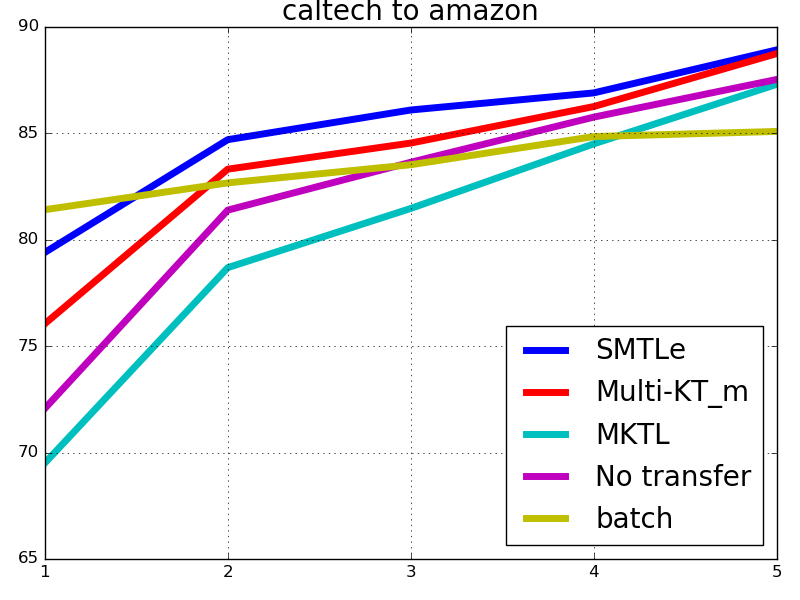
\includegraphics[width=0.3\textwidth]{fig/caltechtoamazon.png}\label{a}
}
\subfigure{
    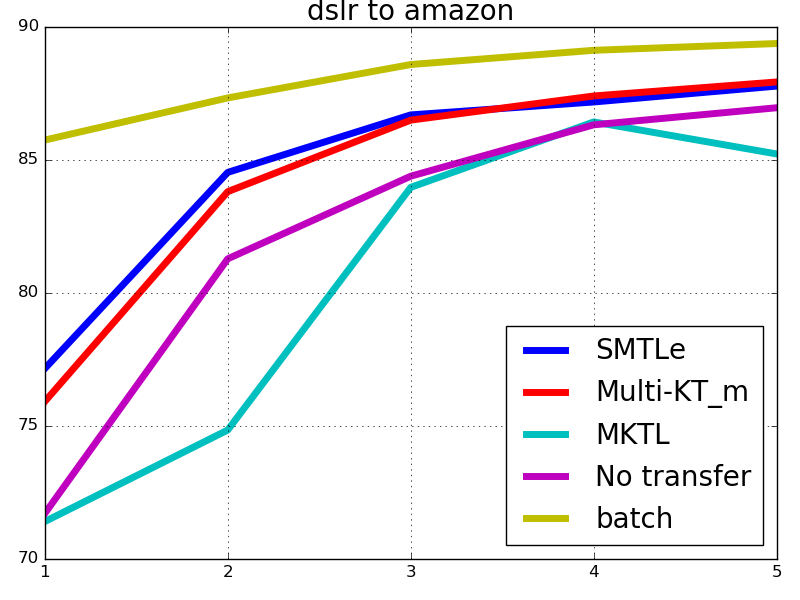
\includegraphics[width=0.3\textwidth]{fig/dslrtoamazon.png}\label{b}
}
\subfigure{
	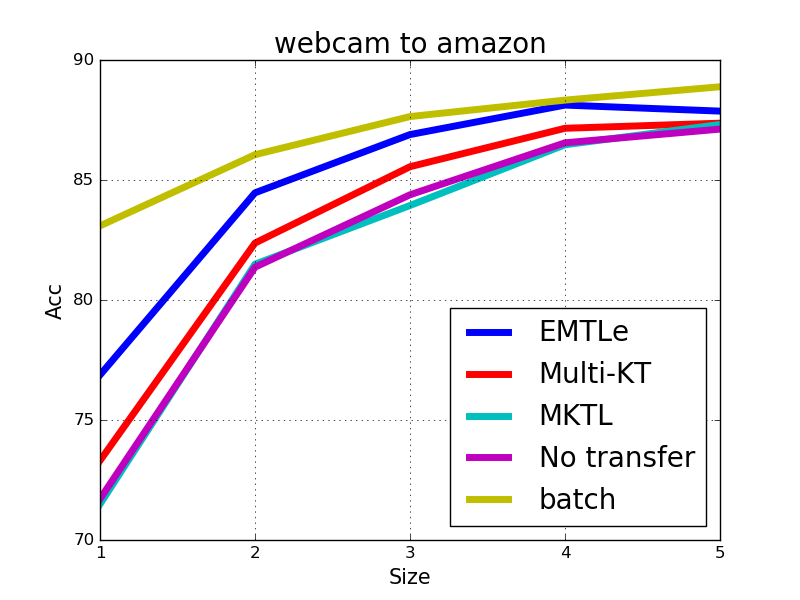
\includegraphics[width=0.3\textwidth]{fig/webcamtoamazon.png}\label{c}
}\\
\subfigure{
	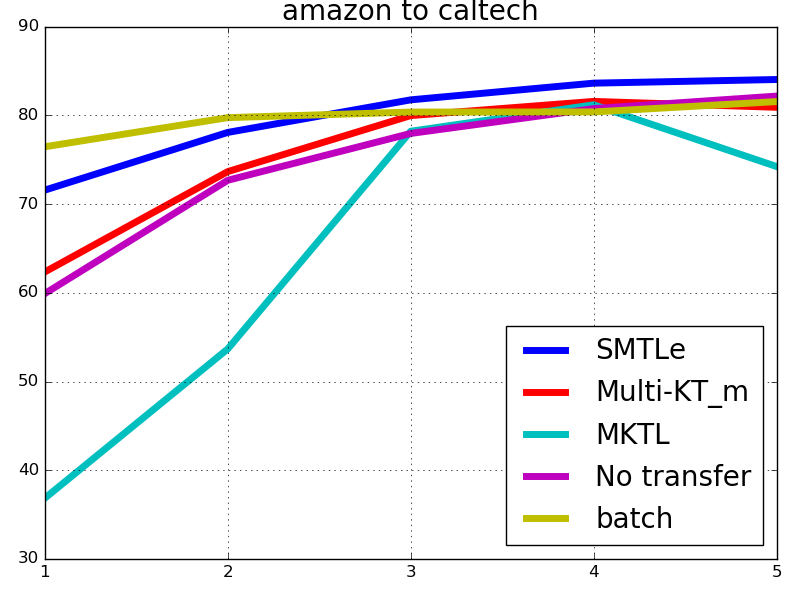
\includegraphics[width=0.3\textwidth]{fig/amazontocaltech.png}\label{d}
}
\subfigure{
	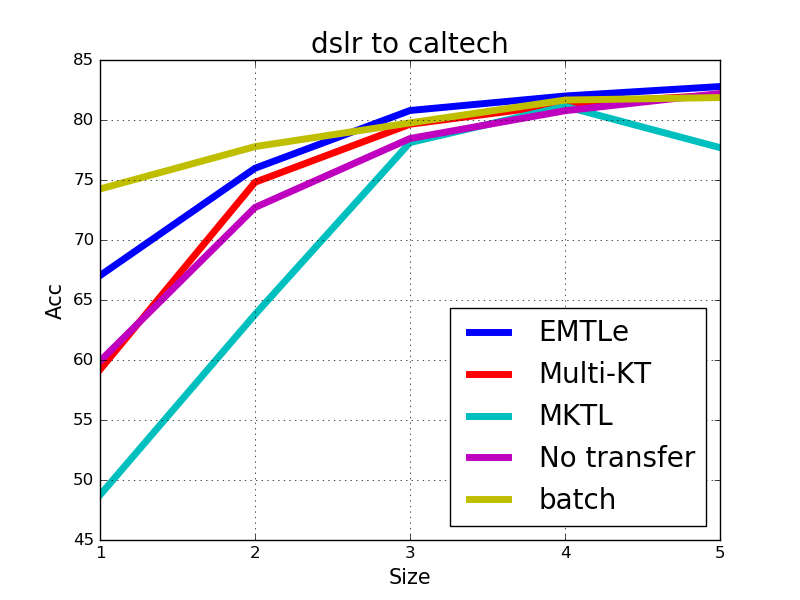
\includegraphics[width=0.3\textwidth]{fig/dslrtocaltech.png}\label{e}
}
\subfigure{
	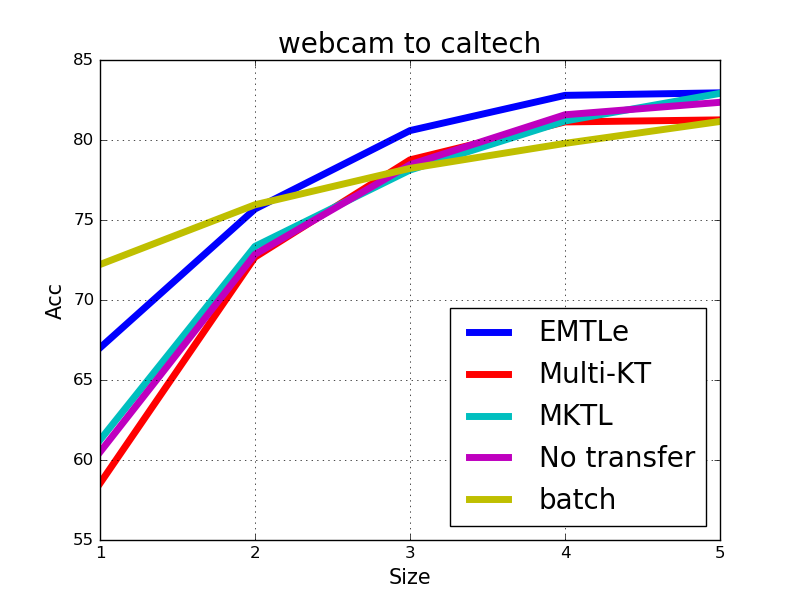
\includegraphics[width=0.3\textwidth]{fig/webcamtocaltech.png}\label{f}
}\\
\caption{HTL domain adaptation experiment results. 5 different sizes of target training sets are used in each group of experiments.}
\label{fig:exp}
\end{figure}